%!TEX root = ../thesis.tex
%*******************************************************************************
%****************************** Second Chapter *********************************
%*******************************************************************************
\graphicspath{{Chapter2/Figs/Vector/}{Chapter2/Figs/}}

%%%%%%%%%%%%%%%%%%%%%%%%%%%%%%%%%%%%%%%%%%%%%%%%%%%%%%%%%%%%%%%%%%%%%%%%%%%%%%%%
% Encoding Locations
%%%%%%%%%%%%%%%%%%%%%%%%%%%%%%%%%%%%%%%%%%%%%%%%%%%%%%%%%%%%%%%%%%%%%%%%%%%%%%%%
%
\chapter{Encoding Locations}
\section{Introduction}

To answer in what way locations can be represented to be universally interpretable, the definition of a location must be well understood. Encoding of locations has historically been of great importance, and is always being modernized. This chapter aims to find the best method of representing locations that is universally interpretable and most importantly usable in this project. Locations, plurally, suggesting that more than one location should be encoded. This is where the challenge lies.

%%%%%%%%%%%%%%%%%%%%%%%%%%%%%%%%%%%%%%%%%%%%%%%%%%%%%%%%%%%%%%%%%%%%%%%%%%%%%%%%
% A Brief History Of Geographic Locations
%%%%%%%%%%%%%%%%%%%%%%%%%%%%%%%%%%%%%%%%%%%%%%%%%%%%%%%%%%%%%%%%%%%%%%%%%%%%%%%%
%
\section{A Brief History Of Geographic Locations}
A location is roughly described as a place or position. Throughout history, various navigational techniques and tools like the sextant, nautical chart and marinner's compass were used, measuring the altitude of the North Star to determine the latitude $\phi$, in conjunction with a chronometer to determine the longitude $\lambda$ of a location on the Earth's surface. \mynote{galileo}

\begin{figure}[htbp!]
	\centering
	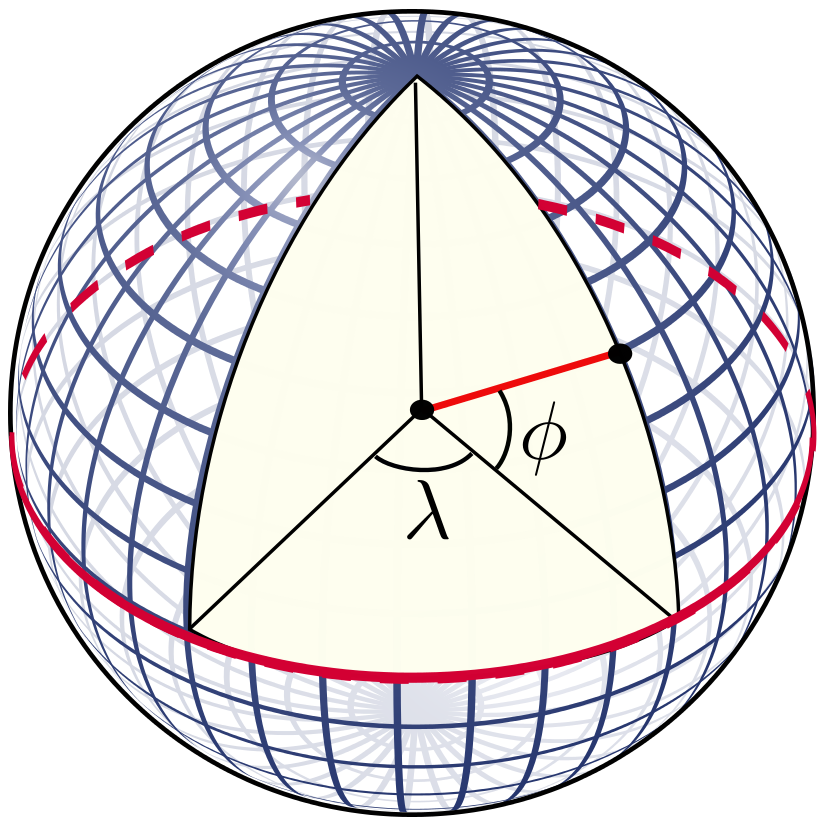
\includegraphics[width=.2\textwidth]{LatLngSphere}
	\caption[LatLngSphere]{A perspective view of the Earth showing how latitude and longitude are defined on a spherical model.}
	\label{fig:latlngsphere}
\end{figure}

Modern navigation relies on sattelites that are capable of providing information to determine a location with an accuracy of 9 meters. The precision of hybrid methods using cell towers and Wi-Fi Location Services enables precise tracking of modern devices. Latitude and longitude are often referred to as GPS coordinates, as GPS is often used to calculate latitude and longitude by receiving position and time code sequences from at least four sattelites. Addresses are another representation of a location used in navigation. Addresses are easier to communicate than a pair of GPS coordinates, but can be ambiguous, imprecise, inconsistent in format. Addresses commonly make use of Postal Code systems, which have reliably been assigned to geographical areas with the purpose of sorting mail. Although even today, there are countries that do not have a Postal Code system.
A location being roughly described as a place or position, can be decomposed as an abstract term to describe physical or imaginary areas with varying radiusses and shapes. You could prepend 'the location of' to the following terms as an example: America, the birthplace of Sokrates, Wall Street, the center of the universe, the Laryngeal Nerve of the Giraffe, churches in the Netherlands. The final example presents the main challenge before mentioned of this project.

%%%%%%%%%%%%%%%%%%%%%%%%%%%%%%%%%%%%%%%%%%%%%%%%%%%%%%%%%%%%%%%%%%%%%%%%%%%%%%%%
% Useful Location Types
%%%%%%%%%%%%%%%%%%%%%%%%%%%%%%%%%%%%%%%%%%%%%%%%%%%%%%%%%%%%%%%%%%%%%%%%%%%%%%%%
%
\section{Useful Location Types}
While setting up a backlog, a shared knowledge about the terminology used in the issues must be achieved. In the pregame document, the term "area" was defined as a collection of three or more coordinate pairs, or a collection of postal codes. A "point" was defined as one distinct coordinate pair or one distinct postal code. This way a location could either be an area or a point, with which all possibilities are covered. As stated in Appendix \ref{appendix:pregame}, the definition of an area is precise, unambiguous and easy to use in compare in computer programs. A single point may match another single point if it’s the exact same point. A point may be sitting on top of a line or is contained within an area. The only other option is the negation of these statements. Because use cases for lines will be non-existent, points and areas are the proper candidates for spatial queries.

%%%%%%%%%%%%%%%%%%%%%%%%%%%%%%%%%%%%%%%%%%%%%%%%%%%%%%%%%%%%%%%%%%%%%%%%%%%%%%%%
% Requisites of Location types
%%%%%%%%%%%%%%%%%%%%%%%%%%%%%%%%%%%%%%%%%%%%%%%%%%%%%%%%%%%%%%%%%%%%%%%%%%%%%%%%
%
\section{Requisites of Location types}
A taxi company director wants to be able to set price or define discounts from or to a certain location. They would like to define prices based only on departure locations, or only on destination locations, or both. For example: 'to Schiphol, a trip should cost \euro 10,-', or 'from Falke hotels a trip should cost \euro 5,-', or 'from Falke hotels to Schiphol, the km price should be \euro 0,60'. In the current implementation, a record would be stored containing departure location, destination location and price for every combination, where locations were defined as zip codes. Instead, it would make sense to be able to reuse locations after they have been defined once.

%%%%%%%%%%%%%%%%%%%%%%%%%%%%%%%%%%%%%%%%%%%%%%%%%%%%%%%%%%%%%%%%%%%%%%%%%%%%%%%%
% Literature review
%%%%%%%%%%%%%%%%%%%%%%%%%%%%%%%%%%%%%%%%%%%%%%%%%%%%%%%%%%%%%%%%%%%%%%%%%%%%%%%%
%
\section{Literature Review}
\mynote{Potentially add literature review}

%%%%%%%%%%%%%%%%%%%%%%%%%%%%%%%%%%%%%%%%%%%%%%%%%%%%%%%%%%%%%%%%%%%%%%%%%%%%%%%%
% Database Prerequisites
%%%%%%%%%%%%%%%%%%%%%%%%%%%%%%%%%%%%%%%%%%%%%%%%%%%%%%%%%%%%%%%%%%%%%%%%%%%%%%%%
%
\section{Database Prerequisites}
The database must be capable of determining whether a virtual perimeter contains a set of coordinates, more specifically, it must adhere to The Open Geospatial Consortium (OGC) Simple Feature Access ISO 19125-1 \cite{SFA} and ISO 19125-2 \cite{SFS}, including spatial data types, analysis functions, measurements and predicates for this requirement, or have some comparable implementation. The scenario presented in image \ref{fig:square} should be replicable.

\begin{figure}[htbp!]
	\centering
	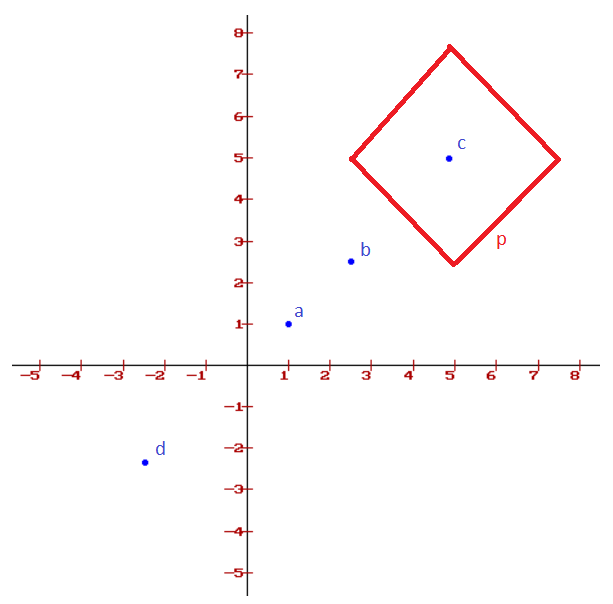
\includegraphics[width=.5\textwidth]{Square}
	\caption[Square]{Four Points, one Polygon p containing Point c.}
	\label{fig:square}
\end{figure}

\subsection{OpenGIS Compatible databases}
MYSQL’s innate integrity is a good reason to opt for a full MYSQL database setup. MariaDB is a fork of MYSQL that performs better according to benchmarks, however they don’t always translate to real life situations. It’s easy to migrate from MYSQL to MariaDB, so choosing MYSQL at first could be preferable as an instance of MYSQL is already used at TaxiID. PostgreSQL offers a spatial database extender for that is OpenGIS compliant called PostGIS that adds support for geographic objects and location queries.

All spatial data types inherit properties such as type and spatial reference identifier (SRID). For rigorous documentation, both PostGIS documentation \cite{PostGIS} and MYSQL documentation \cite{MySQL} could be consulted. When a generic geometry column, or point column is created, points can be inserted as shown in snippet \ref{lst:sql-insert-points} and \ref{lst:sql-insert-polygon} \\

\begin{multicols*}{2}
\begin{lstlisting}[caption={Insert four points}, label={lst:sql-insert-points}]
	START TRANSACTION;
	SET @a = ST_GeomFromText('POINT(1 1)');
	INSERT INTO point (point) VALUES (@a);
	SET @b = ST_GeomFromText('POINT(2.5 2.5)');
	INSERT INTO point (point) VALUES (@b);
	SET @c = ST_GeomFromText('POINT(5 5)');
	INSERT INTO point (point) VALUES (@c);
	SET @d = ST_GeomFromText('POINT(-2.5 -2.5)');
	INSERT INTO point (point) VALUES (@d);
	COMMIT;
\end{lstlisting}
\begin{lstlisting}[caption={Insert polygon}, label={lst:sql-insert-polygon}]
	START TRANSACTION;
	# First and last point must be the same
	SET @a = PolygonFromText('POLYGON((2.5 5,5 7.5,7.5 5,5 2.5,2.5 5))');
	INSERT INTO polygon (polygon) VALUES (@a);
	COMMIT;
\end{lstlisting}
\end{multicols*}


It is evident that c is contained in p. To determine which points are contained in p, the function as seen in Snippet \mynote{Add ref to snippet} can be used, which returns the point with coordinates $[5, 5]$ as expected.

\mynote{Make multicol}
\begin{lstlisting}
	// All points contained in polygon
	SELECT ST_ASTEXT(POINT)
	FROM POINT
	WHERE
	ST_CONTAINS(
			(
				SELECT POLYGON
				FROM POLYGON
				WHERE id = 1
			),
			POINT
		)

	// All polygons containing point
	SELECT ST_ASTEXT(POLYGON)
	FROM POLYGON, POINT
	WHERE
		POINT.id = 3 AND ST_CONTAINS(
			POLYGON.polygon,
			POINT.point
		)
\end{lstlisting}

\subsection{OpenGIS Incompatible databases}
MongoDB doesn’t offer OpenGIS implementations but has geospatial query operators that may provide enough functionalities for current requirements \mynote{Add ref to Geospatial Query Operators — MongoDB Manual 3.6}. The argument for choosing one over the other depends on the vast differences between SQL and NoSQL, next to performance and extensiveness of geospatial features. The setup displayed in image \mynote{Add ref to image} is recreated in MongoDB using queries shown in snippet \mynote{Add ref to snippet}.

\begin{Verbatim}[fontsize=\scriptsize]
	db.point.insertMany([
	{ shape: { type: "Point", coordinates: [1, 1] } },
	{ shape: { type: "Point", coordinates: [2.5, 2.5] } },
	{ shape: { type: "Point", coordinates: [5, 5] } },
	{ shape: { type: "Point", coordinates: [-2.5, -2.5] } },
	])

	db.polygon.insert({
	shape: {
	type: "Polygon",
	coordinates: [ [ [2.5, 5], [5, 7.5], [7.5, 5], [5, 2.5], [2.5, 5] ] ]
	}
	})

	db.point.createIndex({ ‘shape’: '2dsphere' })
	db.polygon.createIndex({ ‘shape’: '2dsphere' })
\end{Verbatim}

\mynote{Make multicol}
\begin{Verbatim}[fontsize=\scriptsize]
	// All points contained in polygon
	var p = db.polygon.find({})

	db.point.find({
	shape: {
	$geoWithin: {
	$polygon: [
	[2.5, 5],
	[5, 7.5],
	[7.5, 5],
	[5, 2.5],
	[2.5, 5]
	]
	}
	}
	})

	// All polygons containing point
	var p = db.point.findOne({ coordinates: [5, 5] })

	db.polygon.find({
	shape: {
	$geoIntersects: {
	$geometry: {
	type: "Point",
	coordinates: [5, 5]
	}
	}
	}
	})
\end{Verbatim}

Next to database solutions for this requirement, services exist that are capable of geofencing. Although these services may not be free, and the added dependencies restrict extensibility.

%%%%%%%%%%%%%%%%%%%%%%%%%%%%%%%%%%%%%%%%%%%%%%%%%%%%%%%%%%%%%%%%%%%%%%%%%%%%%%%%
% Performance and Clustering Trade-offs
%%%%%%%%%%%%%%%%%%%%%%%%%%%%%%%%%%%%%%%%%%%%%%%%%%%%%%%%%%%%%%%%%%%%%%%%%%%%%%%%
%
\section{Performance and Clustering Trade-offs}
Agarwal and Rajan state that NoSQL take advantage of cheap memory and processing power, thereby handling the four V’s of big data more effectively,
but lack the robustness over SQL databases \mynote{Add reference to Agarwal and Rajan}. The report dives deeper into spatial queries and concludes that their tests suggest that MongoDB performs better by an average factor of 10, which increases exponentially as the data size increases, but lack many spatial functions that OpenGIS supports. Although improvements have been made \mynote{Add reference to Geospatial Performance Improvements in MongoDB 3.2,” MongoDB} after the cited paper Schmid et al. 2015 \mynote{Add ref to Stephan Schmid Eszter Galicz} was published. The team argues that clustering is much easier in MongoDB, which may be important in the future when the company grows. As the required functionalities exist in both SQL and NoSQL, it is beneficial to opt for MongoDB for its performance and alignment with the teams experience. Although if robustness is desired, or extra GIS functionalities required, SQL should be taken into consideration.


In what way can locations be represented to be universally interpretable?
\begin{enumerate}
	\item Which types of locations should be distinguished?
	\item What are the main differences between postal systems used around the globe?
	\item Can postal codes be abstracted to geospatial data while retaining the same usefulness in the system?
	\item How can different types of locations be effectively stored in a database?
\end{enumerate}
